%Section ----------------------------------------------------------------------------------------------------------------------------------------------------
\newpage
\section{Research plan}  
\label{S:work_plan} 


%--------------------------------------------------
\subsection{Overview}
%--------------------------------------------------

The body of this thesis will be approached as a number of discrete research problems; connected along a conceptual path branching from the preceding Literature Review [Section \ref{S:REVIEW}].\\
Several of the investigations will developed to form viable independent journal publications.  Progress towards a coherent thesis will be guided by the goal of successively creating a series of peer-reviewed publications.\\




An overview of the plan is provided by the following sequence of questions.   
% \begin{mdframed}[hidealllines=true,backgroundcolor=yellow!30]
\BoxBegin
\begin{enumerate}
\item Does coastal sea level from a 0.1 degree B-grid \OGCM{} have physical meaning, and with what limitations? 
	\par[pg \pageref{S:plan_whichcell}]
\item How is the surface height signature of coastally trapped waves represented in \BL{} and why? 
	\par[pg \pageref{S:plan_CTW}]
\item Is there any tidal component in the sea level forecast by this nominally nontidal system and why?
	\par[pg \pageref{S:plan_nontidal_tidal}]
\item How can standard harmonic tidal analysis be approached when the end-use is aggregation with dynamic models?
	\par[pg \pageref{S:plan_insitu_analysis}]
\item Can explicit resolution of tidal physics within and \OGCM{} realistically provide any benefit for coastal sea level?
	\par[pg \pageref{S:plan_OFAMR}]
\item Can a regional tidal model be optimised for use in connection with a tide resolving regional \OGCM{}?
	\par[pg \pageref{S:plan_OTIS}]
\item Is a tide resolving \OGCM{} sensitive to the details of tidal body forcing and can the formulation be improved?
	\par[pg \pageref{S:plan_bodyforcing}]
\item And finally, can the proceeding work inform an initial discussion of the implications of explicit tidal resolution for data assimilation?
	\par[pg \pageref{S:plan_DA}]
\end{enumerate}
%\end{mdframed}
\BoxEnd


%----------------------------------------------------------------------------------------------------------------------------------------------------
%----------------------------------------------------------------------------------------------------------------------------------------------------

\newpage
\subsection{Coastal sea level signal from a 0.1 degree B-grid \OGCM{}}
\label{S:plan_whichcell}
\subsubsection{Problem and motivation}

% intro
Although nominally a blue-water forecasting system, the representation of coastal phenomena in \BL{} has become a topic of increasing operational interest.\\
Initially, this interest was restricted to visual inspection of forecast daily average SLA maps; an  output configuration reflecting the systems target of mesoscale eddies.   Subsequent quantitative assessment \citep{Taylor:2010ud} has been restricted to observations from coastal tide gauges.  Tide gauges being essentially the only observation platform available for routine sea level skill evaluation \BL{}.\\



% setup current evaluation
After several years of maturing interest it is now relevant to re-evaluate exactly how to map the gridded model output to insitu coastal locations. This is a non-trivial matter at the cross-over of representational limits of both the model and observations.\\
Fundamental to this problem is that geographic locations of tide gauges do not coincide exactly with the coastal boundary of the \OGCM{}.  The numerical coast is a key discontinuity represented by a land/sea mask in gridded space.  
\BoxBegin{}
Given that \BL{} uses a staggered Arakawa B-grid at 0.1 degree spacing, can the output be meaningfully mapped to real coastal locations and with what limitations? Is extrapolation valid and why?\\
\BoxEnd{}
All comparisons made to date have utilised a 'nearest coastal neighbour' approach; a choice to directly map the tide gauge location to the geographically closest tracer cell adjacent to the models land/sea interface.  



Closer inspection of the \BL{} configuration has brought certain aspects of model to the fore that invite reconsideration of the 'nearest closest neighbour' approach, namely;
\begin{inparaenum}[(a)]
\item numerics of lateral boundary conditions;
\item split explicit solver scheme;
\item smoothing and suppression of the b-grid checkerboard null mode.
\end{inparaenum}
In addition, since the earlier studies, access to tide gauge data has expanded and recent configurations of \BL{} have provided higher temporal frequency outputs (now 3 hourly averages).\\


\begin{figure}[!h]
	\centering
%	\subfloat[Illustration of Arakawa B-grid overlaid on the coastline represented (black).  Sea level is located at `T' cells whereas velocity is at the staggered `U' cells.  Geographic tide gauge locations can fall beyond the nominal spatial coverage of the model ocean.]{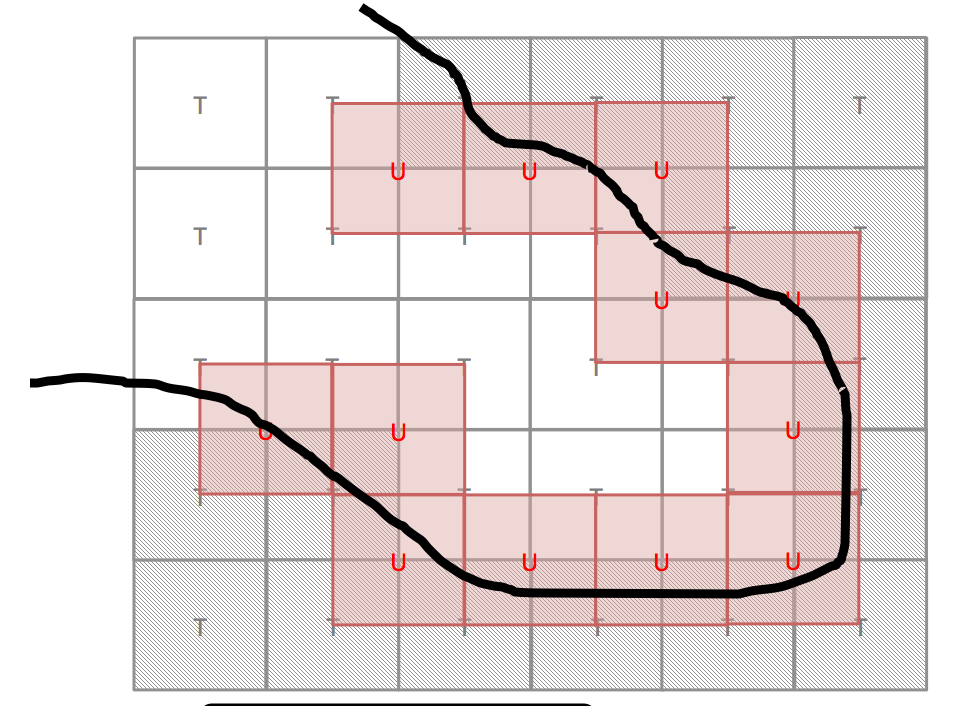
\includegraphics[width=80mm]{figures_3/coastal_masking.png}}\\
	\subfloat[Spatial extent of \OGCM{} T-cells and location of two coastal tide gauges; the possible correspondence of modeled and observed sea level must be subject to limitations]{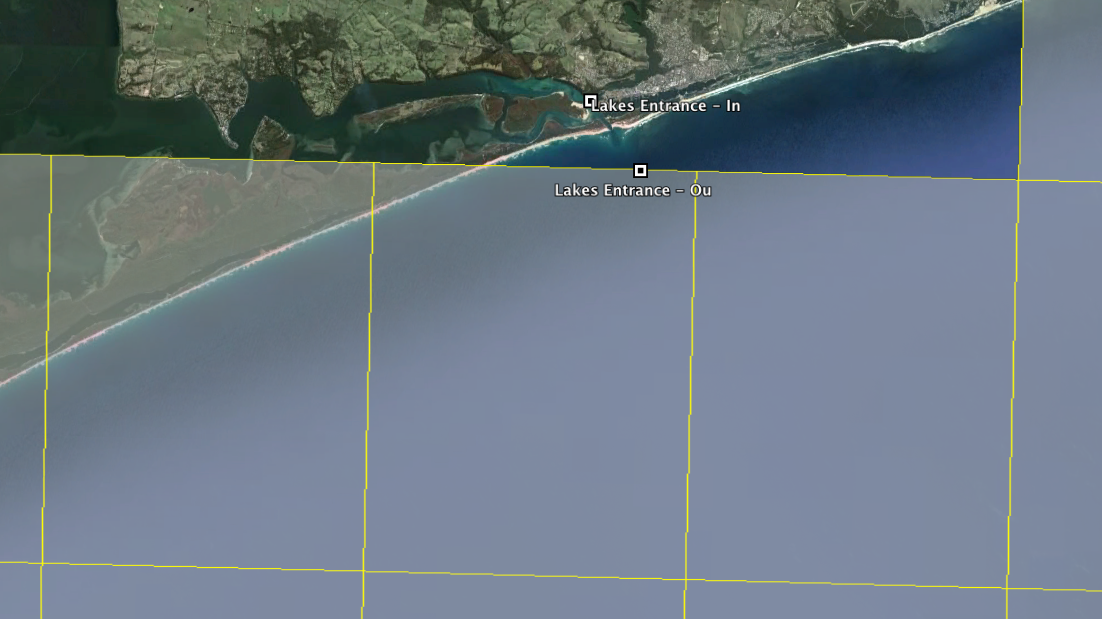
\includegraphics[width=110mm]{figures_3/OFAM_lakes_entrance.png}}\\

	\subfloat[\MOM{} numerical stencils of notable relevance to grid scale noise]{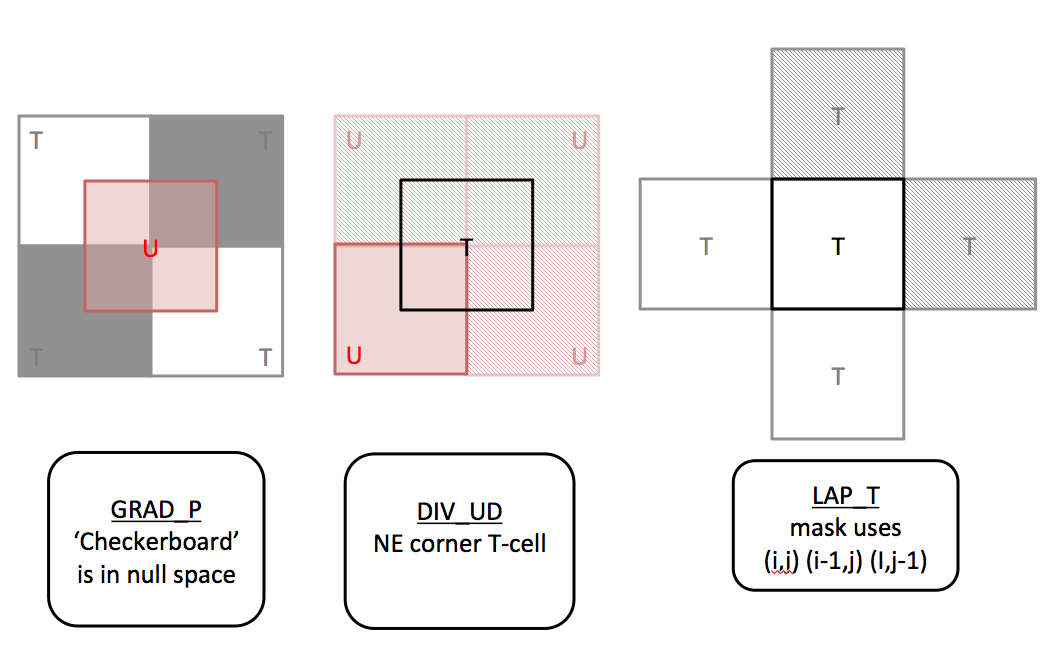
\includegraphics[width=100mm]{figures_3/mom_BT_stencils_extra.png}}
	%\caption{}
	\label{fig:cells_coast}
\end{figure}

\subsubsection{Data sources}
Attention will be restricted to \BL{} behind real time analysis data - so as to set aside questions of forecast skill and focus on spatial representation.\\
Operational output from a neighbourhood about each nominal location will be extracted for the history of the present operational version. \\
Observations will be taken from a subset of those tide gauges that routinely stream data to the \BOM{} (or have the potential to).



\subsubsection{Method outlook}
Primarily this investigation is an empirical comparison of tide gauges observations to a neighbourhood of grid cells.\\
A subset of focus locations will be chosen to specifically explore questions of B-grid noise and the effects of unresolved embayments.   This subset will include: Outer Harbour in SA and Port Phillip Bay in Vic.\\  
Guided by an exposition of relevant numerical operators, a series of mapping methods will be empirically evaluated.   Ultimately this study aims to recommend the single best method for sea level forecast aggregation.




%analytical discussion - BCs, scales, \\
%empirical evaluation:
%nearest any\\
%nearest coastal\\
%weighted combo\\
%filtered ... 

\newpage
\subsection{Propagating coastal surface signal in an \OGCM{}: Australia's East Coast}
\label{S:plan_CTW}

\subsubsection{Problem and motivation}
Coastally trapped waves (CTW) are a phenomena of special interest to operational sea level forecasting in Australia. \\
Anecdotally, \BL{} represents propagating coastal sea level signals which in principle can provide a valuable addition to forecast guidance used within the \BOM.  The extent to which freely propagating CTWs are skilfully forecast and why is not well understood - especially with regard to the extension of the coastal wave guide around Australia's East coast.\\



Powerful surface-apparent CTWs are characteristic of the Southern Coast of Australia and commonly propagate eastward at similar rates to the forcing weather system \citep{Taylor:2009vw}.\\
For this study, regional focus is restricted to the \emph{East Coast} for the following reasons:
\begin{inparaenum}[(a)]
\item extensive discussion of East Coast CTWs in the scientific literature (though typically focussed on subsurface currents);
\item well spaced coastal tide gauge array;
\item indications the \BL{} skill degrades towards the North and within the GBR;  
\item expectation that freely propagating modes may be identifiable in this region;
\item operational impact due to population density.
%\item opportunity to utilise the \ER{} model.
\end{inparaenum}


\subsubsection{Data sources}
Sea level anomaly has been compiled from operational \BL{} analyses during the Austral winter of 2012, a period with no system changes.\\  
Tide gauge data available for this region offers a uniquely dense and well-spaced coastal array - in contrast to other parts of Australia.   The instruments available for this study are operated by the Bureau of Meteorology, Manly Hydraulics Laboratory and the Queensland Department of Environment and Heritage Protection.  Locations included are indicated in Figure \ref{fig:tide_gauges}.\\

\begin{figure}[!h]
	\centering
	\subfloat[tide gauges] {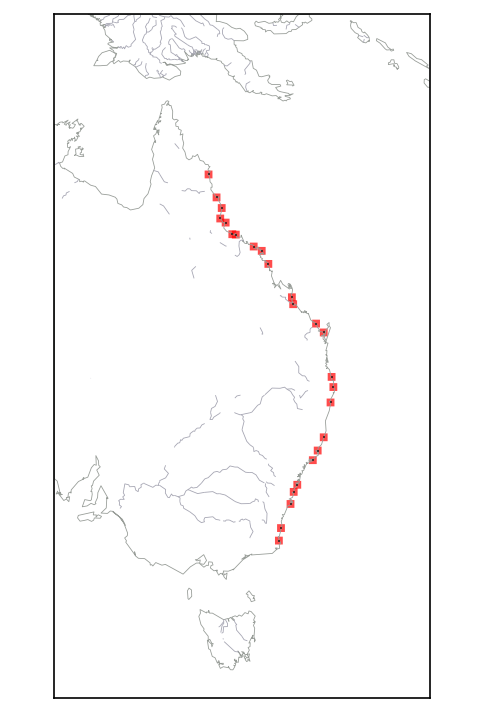
\includegraphics[width=40mm]{figures_3/plot_locations_Australia.png}}
	\subfloat[Illustration of spatial HEOF modes derived from observation array]  {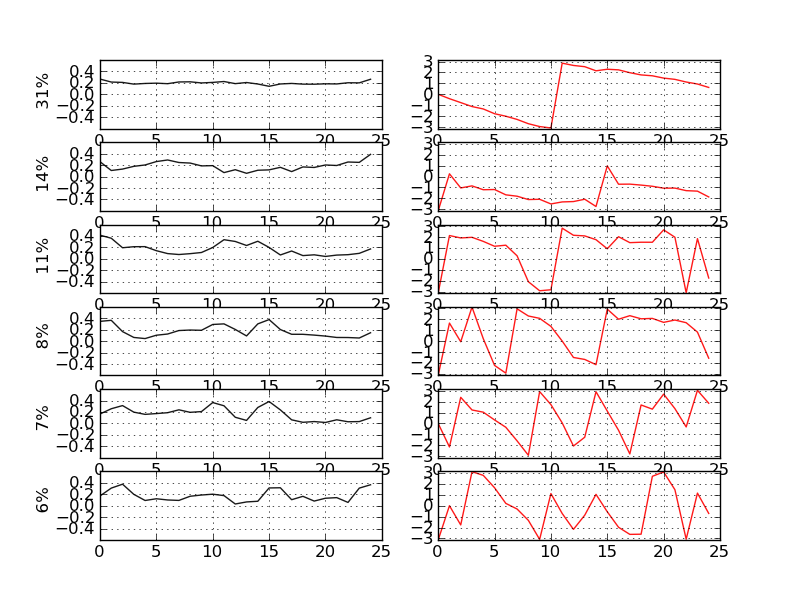
\includegraphics[width=80mm]{figures_3/HEOF_modes_obs.png}}\\
	%\subfloat[Approximate along-shore distance]  {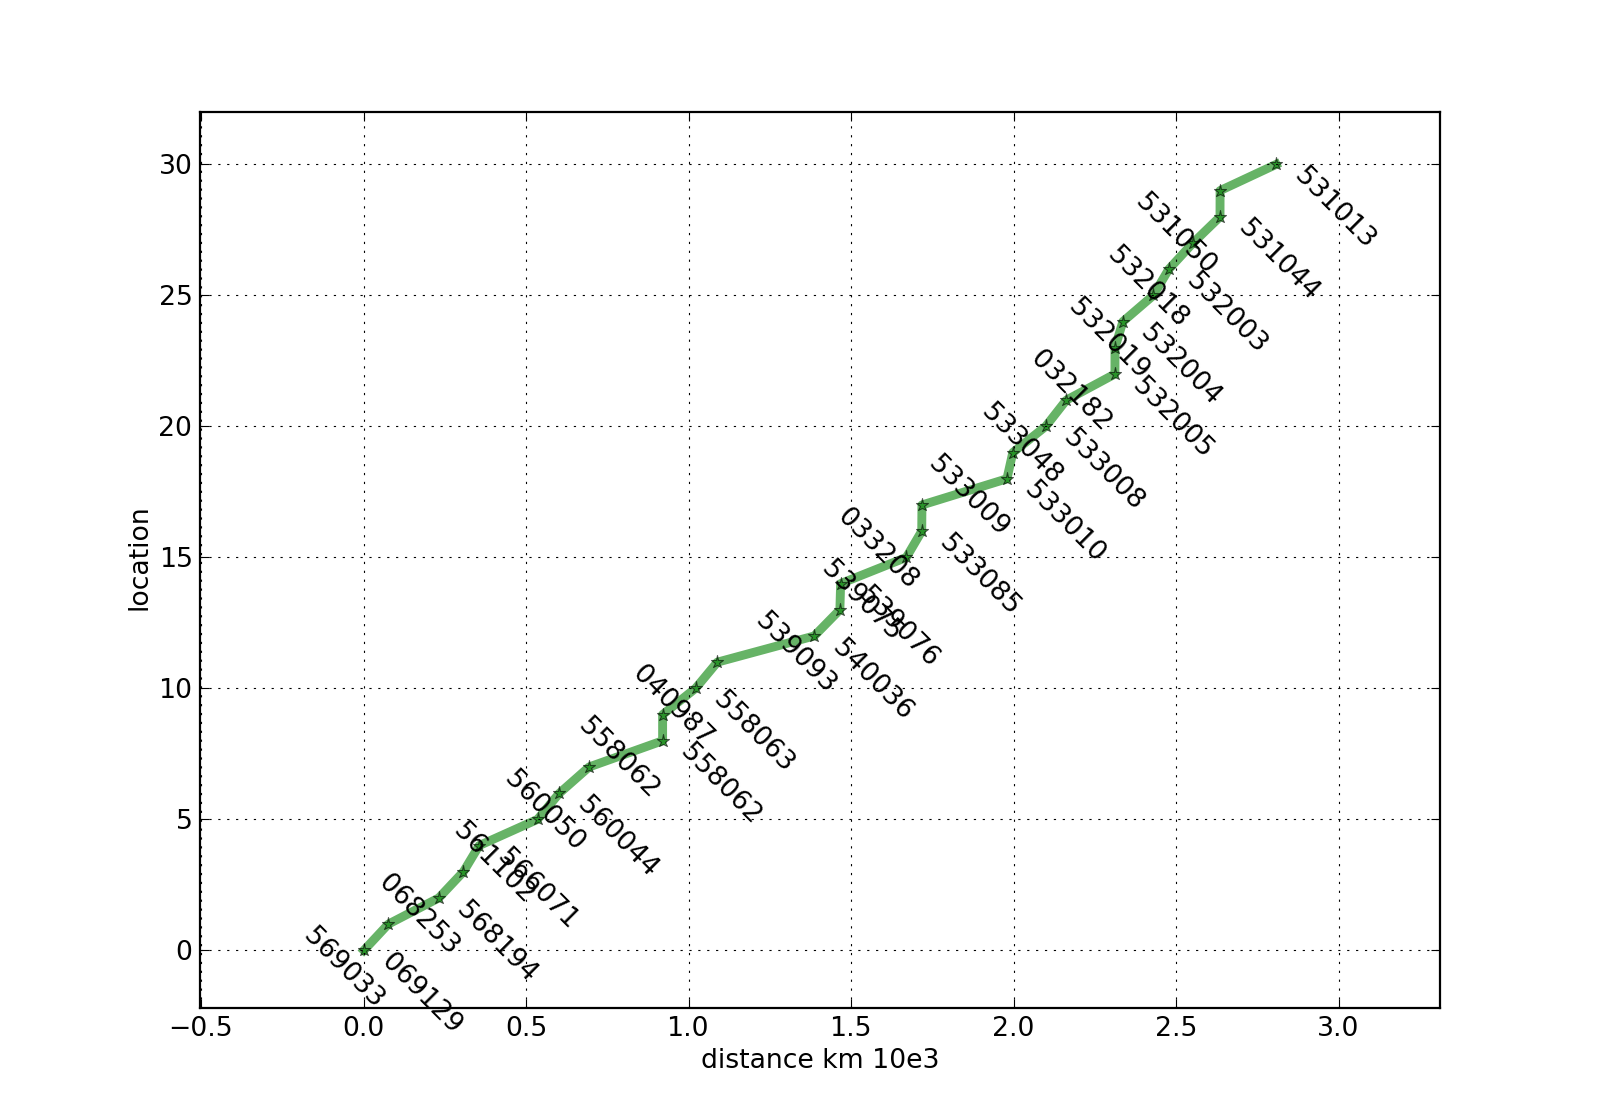
\includegraphics[width=120mm]{figures_3/plot_station_distance.png}}\\
	\caption{Observation locations}
	\label{fig:tide_gauges}
\end{figure}

Depending on availability, simulations from higher resolution ocean models produced by the \BOM{} may be accessed and used for cross-comparison.


\subsubsection{Method outlook}
In essence this study involves the diagnosis of model performance using observations.  Aspects related to coastal propagation are the primary focus.\\ 
Comparison is not physically meaningful without substantial pre-processing.  In the first instance, the observations will be reduced to a SLA quantity by de-tiding.  Subsequently, a signal decomposition method will be employed in order isolate, quantify and diagnose aspects of coastal propagation.  A Hilbert Empirical Orthogonal Functions (HEOF) technique appears to offer an appropriate perspective in this regard.  Previous discussion of related methods offer some insight [REFS]\\

% steps
Work steps sketch:
\begin{enumerate}
\item Prepare observational dataset - including download of additional quality controlled data from MHL and application of appropriate de-tiding; 
\item Characterise observations by spectral content with regard to spacing along coast;
\item Identify candidate propagation events;
\item Characterise raw model forecast skill at each location;
\item Explore the application of HEOF analysis to data subset: Can HEOF modes identify propagation? Does the decomposition offer any insight into model/obs comparison?
\end{enumerate}




This study aims to understand the specific characteristics and limitations of \BL{} along the East Coast; in light of the literature addressing CTWs.   Ultimately, the results may inform the provision of forecasts and prospective system modifications.



%Questions to be addressed:
%\begin{itemize}
%\item where does \BL{} offer any forecast skill on the East Coast?
%\item can the nature of forecast errors be diagnosed?
%\item can error diagnosis guide forecast interpretation and/or suggest system improvements?
%\end{itemize}



%\item Asses \NWP{} forcing:
%%\subitem Regrid $\tau$ from \AG{} and \AR{} the same \OFAM{} target grid.
%\subitem Any systematic biases in \AG{}?

%\item Decompose $\eta_t(t,lat,lon)$ into approximate categories of locally and remotely forced.  
%\subitem Assess decomposed $eta_t$ skill against observations. 
%\subitem Is the relative impact of local versus remote forcing identifyable?

%\item Compare \BL{} against \ER{} $\eta_t$ for the GBR region. 
%\subitem Is raw skill of \ER{} better than \BL{}?
%\subitem Diagnose difference in \ER{}.  
%\end{enumerate}

%\begin{figure}[!h]%
%	\centering
	%\subfloat[overlaid timeseries of observations and eta] {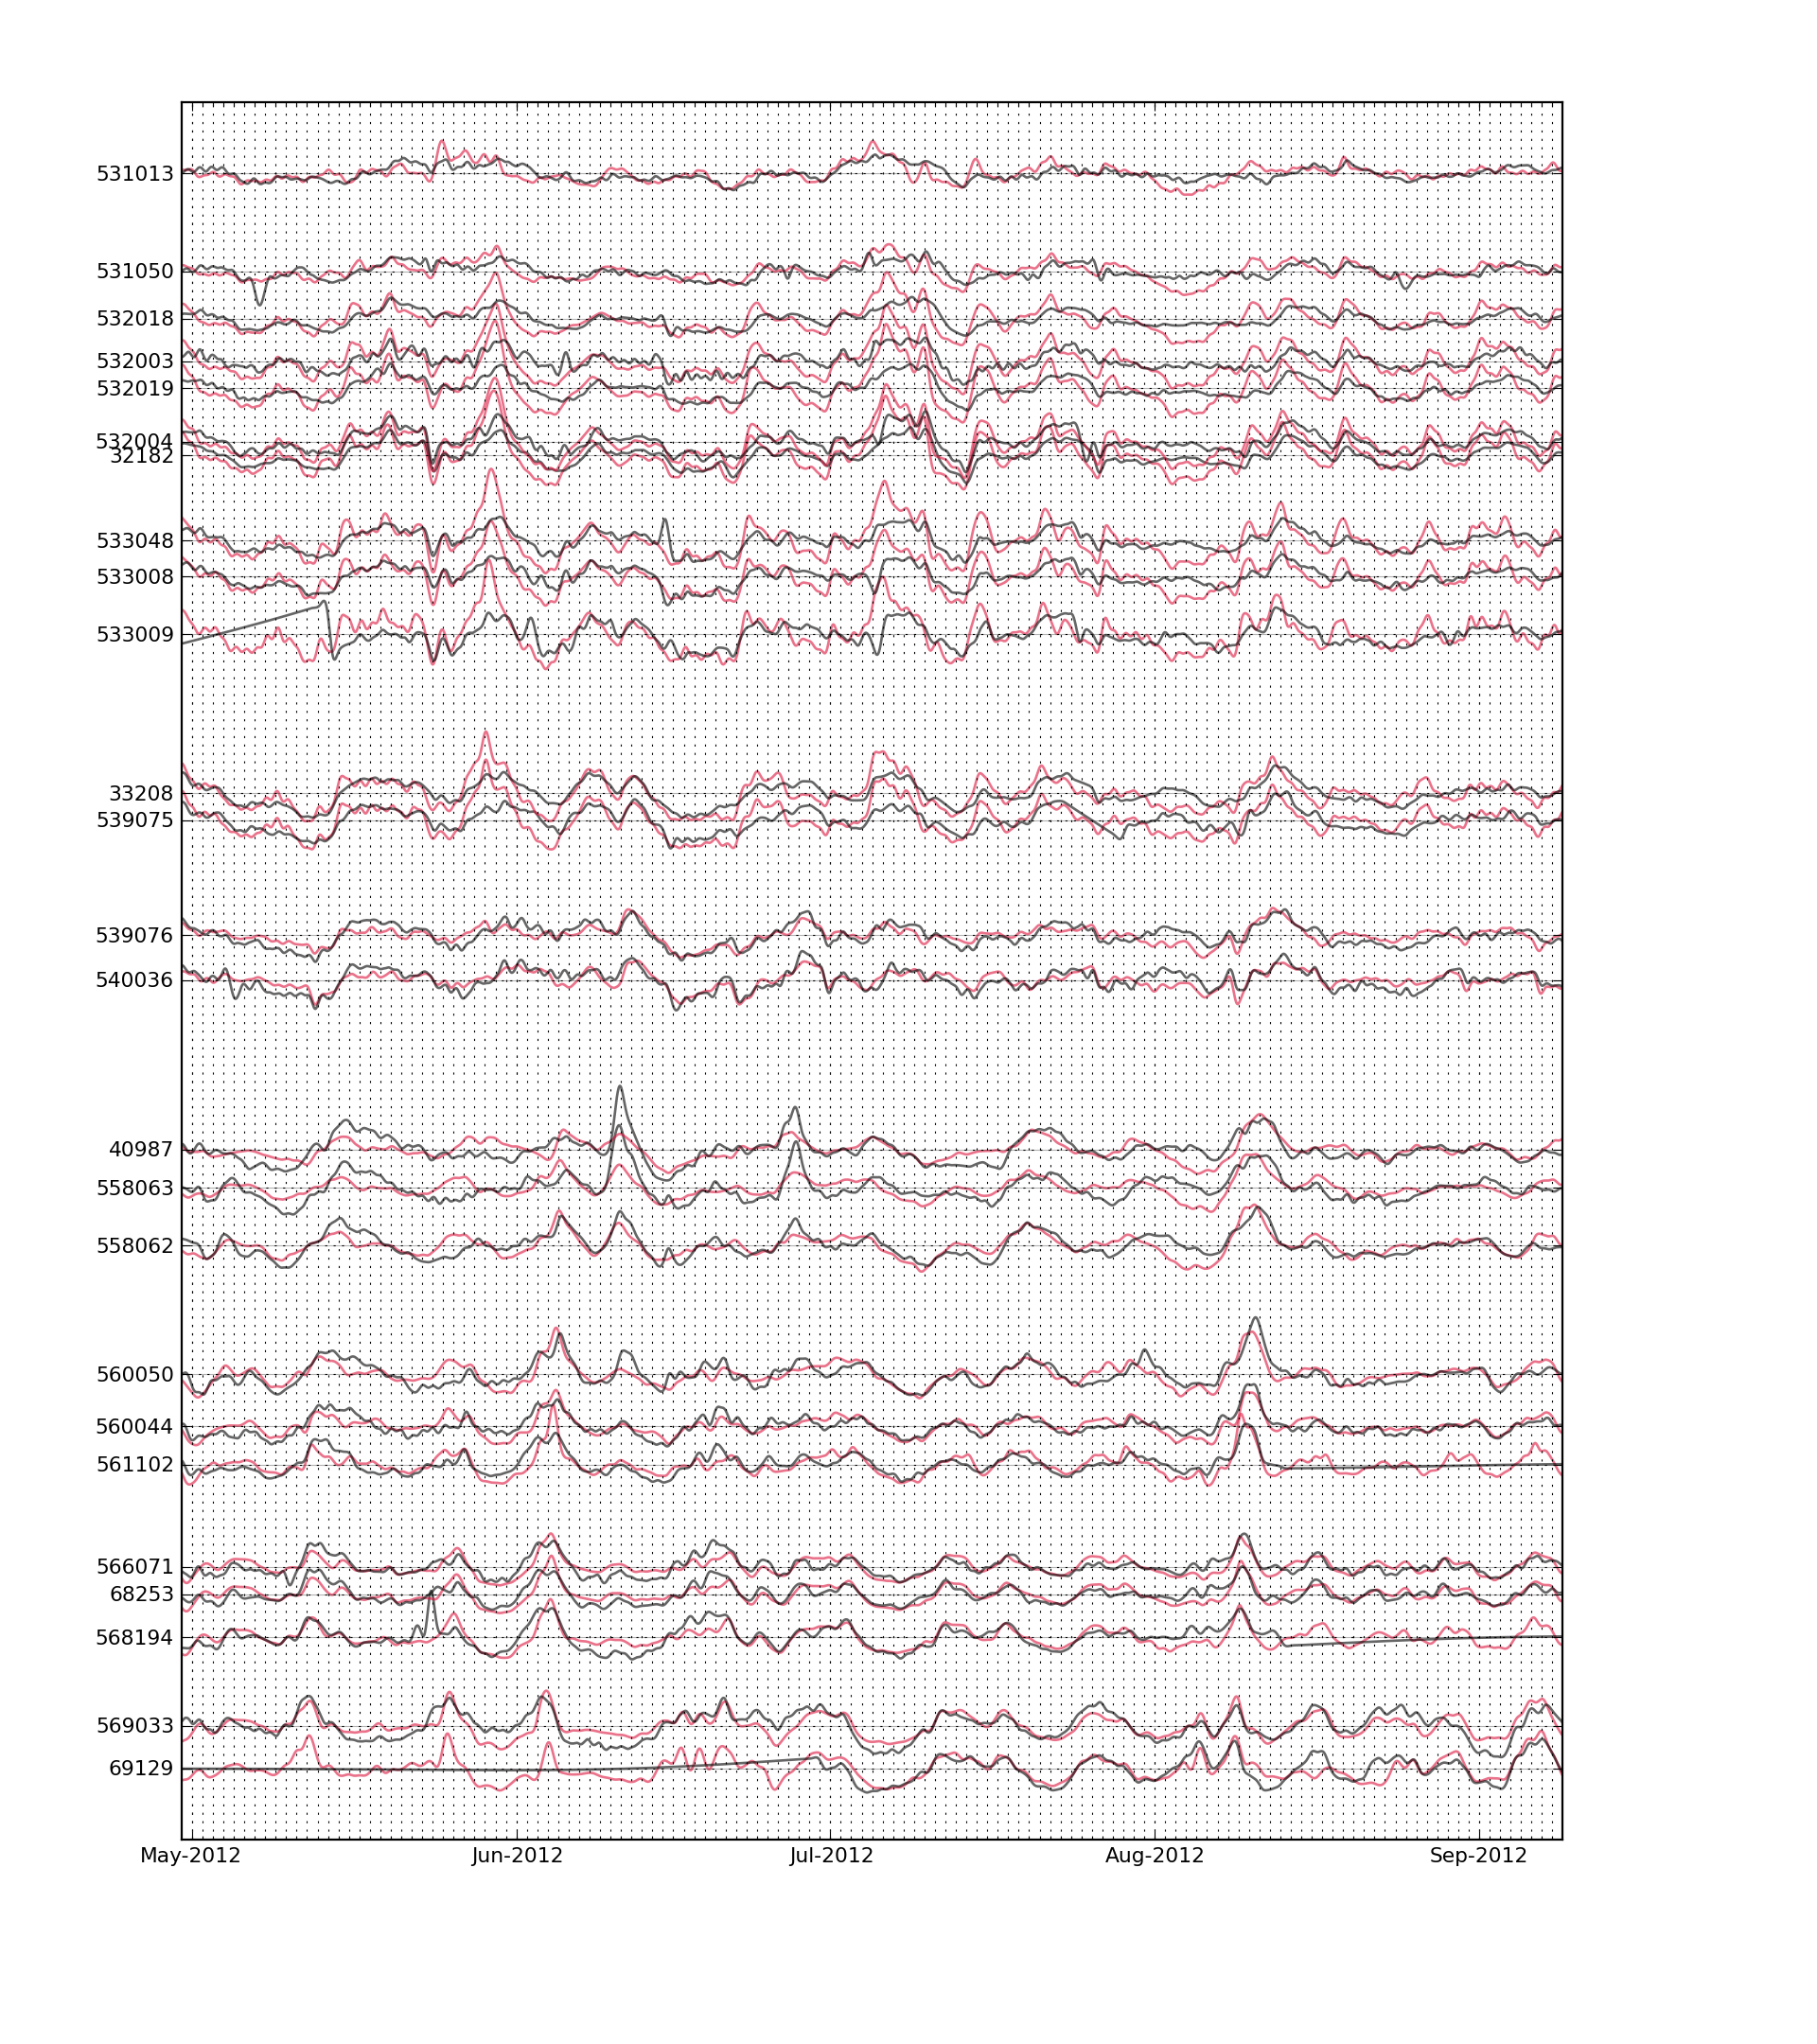
\includegraphics[width=100mm]{figures_3/plot_tsstack_bpass60p0_1p2.png}}\\
%	\subfloat[illustration of spatial HEOF modes derived from observation array]  {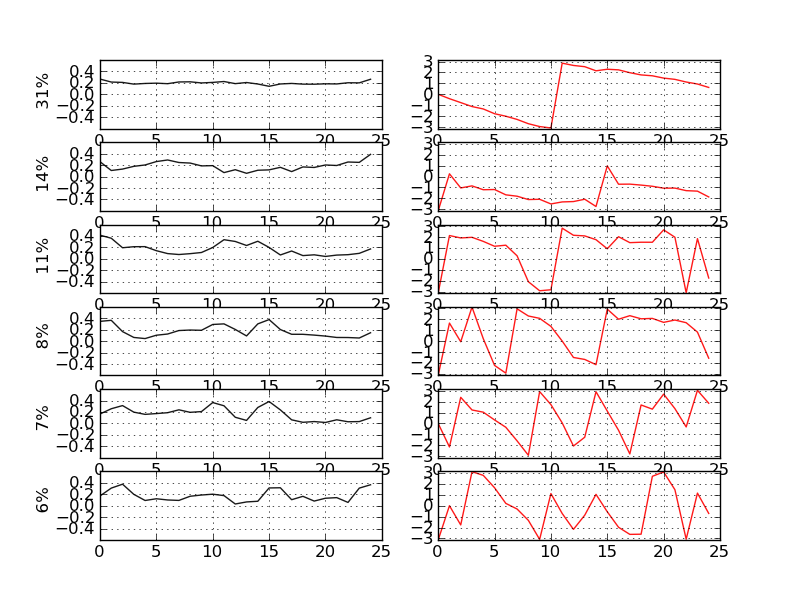
\includegraphics[width=120mm]{figures_3/HEOF_modes_obs.png}}\\
%	\caption{Observation locations}
%	\label{fig:HEOF_overview}
%\end{figure}



\newpage
\subsection{Tidal harmonic analysis of a nontidal \OGCM{}}
\label{S:plan_nontidal_tidal}

\subsubsection{Problem and motivation}
Resolving exactly what constitutes a `tidal' ocean signal is at the core of operational issues raised in the Literature Review [Section \ref{S:REVIEW}].\\
What at first appears to be a question of semantics may in fact have direct implications for the provision of sea level forecasts; especially where heterogeneous forecast systems are aggregated.\\
The premise of this study is that the sea level signal from \BL{} and conventional harmonic prediction are not mutually exclusive.  And if this is in fact the case, that aggregation should take account of this `overlap'.\\



This study aims to identify and understand what `tidal' sea level signals are present in the `nontidal' prediction system.\\
It is expected that this sub-component of the model output will include at least two distinct classes of overlap with conventional harmonic tides:
\begin{itemize}
\item periodic or quasi-periodic `meteorological' tidal constituents;
\item aperiodic `noise' (the turbulent red spectrum) that may contaminate a harmonic analysis. 
\end{itemize}


\subsubsection{Data sources}
Ultimately this study aims to understand \BL{} and inform the application of forecast aggregation.   However, it is anticipated that another directly related simulation will form the basis of this analysis - namely the multi-year \OFAM{} hindcast referred to as `the spinup run'.   In contrast to \BL{} itself, the spinup offers a longer time series produced by a constant configuration and avoids possible complications added by the effects of the data assimilation cycle.  The length of observational records are fundamental to the application of tidal analysis.\\
For comparison, observations from the ABSLMP array of coastal tide gauges [Figure \ref{fig:ABSLMP}] will be employed due to the uniquely accessible uninterrupted historical record.\\
In addition, tidal constituents produced for the Australian National Tide Tables will be referenced where relevant.

\begin{figure}[h]
\begin{center}
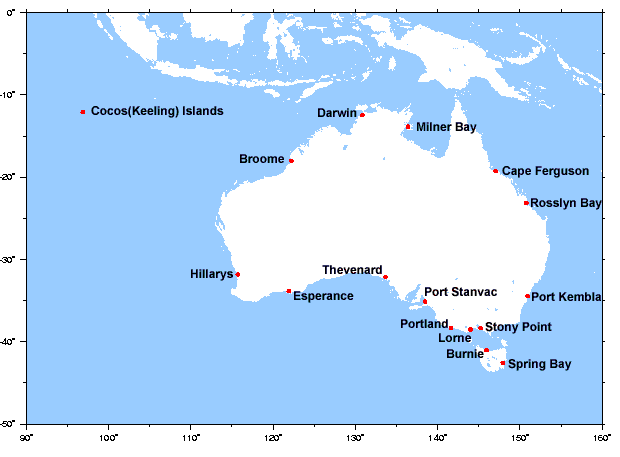
\includegraphics[width=90mm]{figures_3/map_abslmp.png}
\caption{ABSLMP sites with quality controlled data and barometric pressure observations}
\label{fig:ABSLMP}
\end{center}
\end{figure}



\subsubsection{Method outlook}
Timeseries of model output at discrete points will be compiled in the form of pseudo tide-gauge records.  At a minimum the selection of points will be aligned with the ABSLMP  array of tide gauges.  However, if computational resources allow the series of points may be extended to included a full spatial grid across the Australia region. \\

The timeseries fitting problem is formulated:\\
 $\M{A} \V{x}=\V{b}$
 where $\M{A}$ is a matrix of tidal timeseries basis functions, $\V{x}$ is the analysed tidal solution an $\V{b}$ is an observational record. \\
Use of the Singular Value Decomposition (SVD) method described by \citep{Cherniawsky:2011en} facilitates metrics addressing aspects of error and quality of fit.



It is anticipated that the available output frequency of the simulations will be a factor in preparing the data and place limitations on the analysis.   Conventional tidal practice is to analyse instantaneous hourly water level observations.   Simulation data is definitely available as daily averages, and the extent to which the more useful 3-hourly average data is available is to be determined.  Interpolation via an integral variable method is noted as a relevant tool for preparing such model output.\\
Tidal harmonic analysis will be performed on these records with a particular focus on the uncertainty bounds of any fit. It is noted that if \BL{} was in fact naively 'nontidal' then no tidal constituents would be fitted. \\



The results of these analysis will be discussed in light of the following questions: 
\begin{inparaenum}[(a)]
\item does the nominally non-tidal sea level signal project onto a tidal basis?
\item to what extent is this limited by record length and sample frequency?
\item can statistically significant tidal components be expected in \BL{}?
\end{inparaenum}



The result of this investigation will directly inform subsequent questions to be addressed in Section \ref{S:plan_insitu_analysis}\\


















\newpage
\subsection{Tidal harmonics to compliment aggregation with nontidal forecasts}
\label{S:plan_insitu_analysis}

\subsubsection{Problem and motivation}
Tidal harmonic predictions are often not treated as stand-alone forecast products. 
A recently developed scenario is the aggregation of harmonic tides with \BL{} sea level forecasts.\\

Following the discussion in the Literature Review [Section \ref{S:REVIEW}] there is reason to expect that aggregation may require measures to account for the `overlap' between heterogeneous forecast systems.   In fact, developmental aggregated forecasts (eg. Figure \ref{fig:aggregated_fc}) have been produced by modifying standard harmonic predictions.   It is now relevant to understand issues associated with such modifications in greater detail.\\



\begin{figure}[h]
\begin{center}
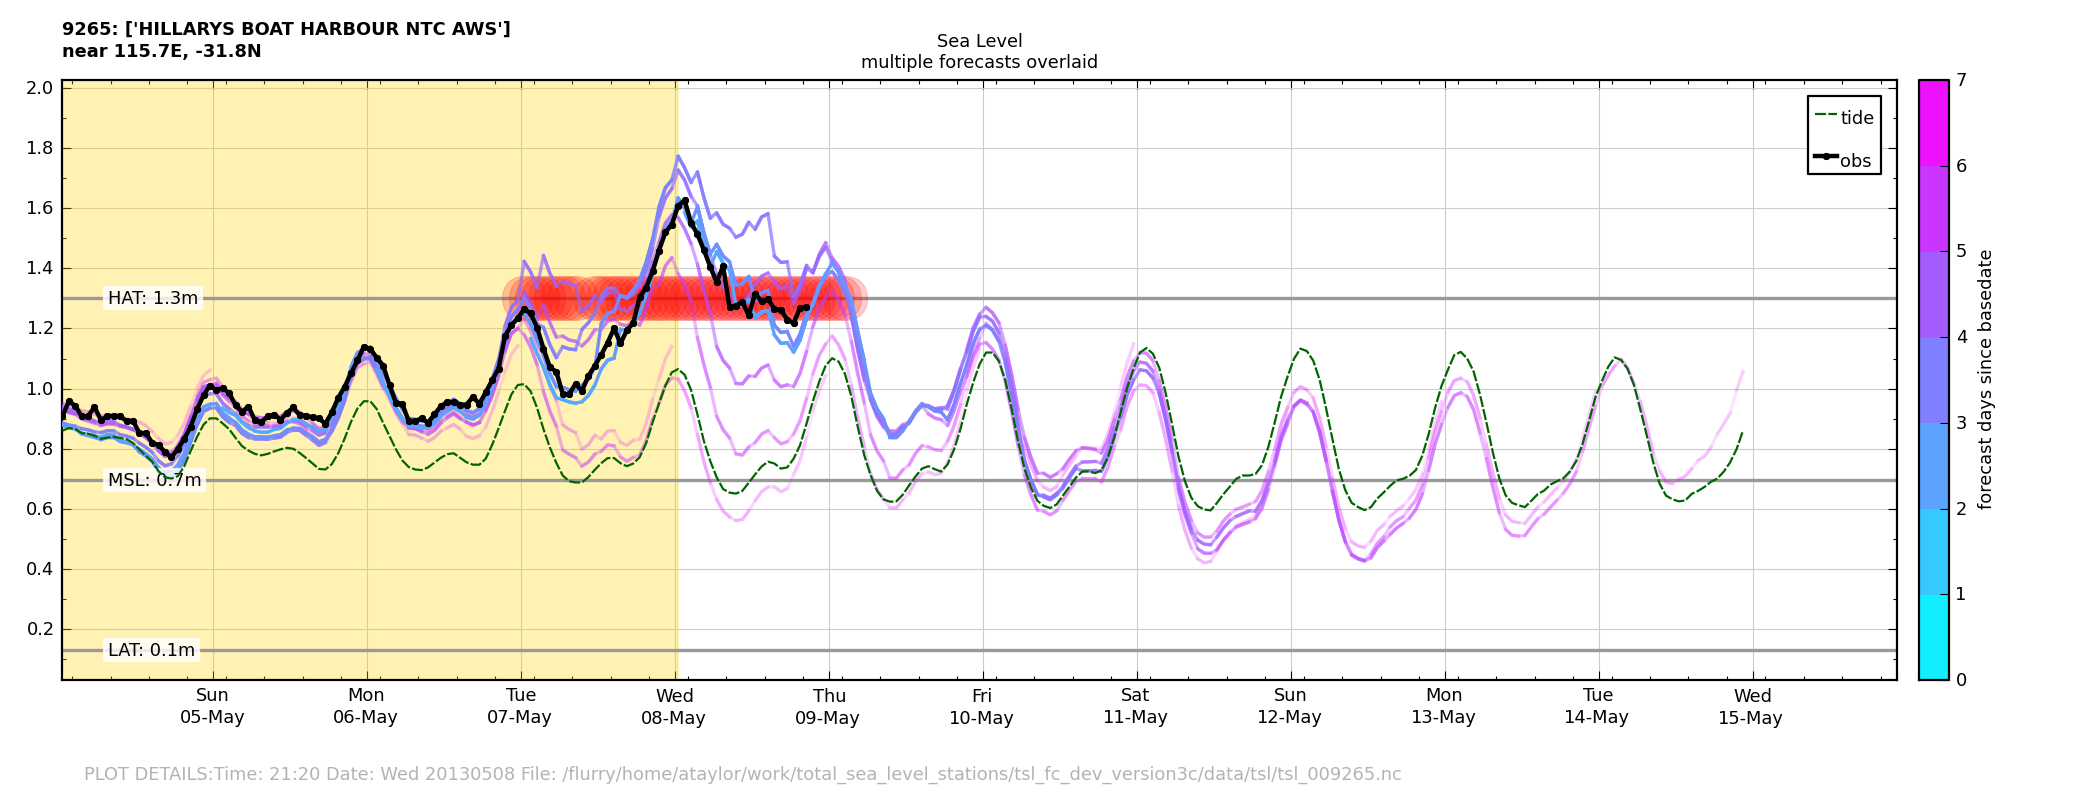
\includegraphics[width=150mm]{figures_3/aggregate_fc_plot_009265.png}
\caption{Aggregated sea level forecast example.   The harmonic tide component has been modified by the removal of certain constituents. Also of note is the spread of lagged-ensemble members related to forecast uncertainty.}
\label{fig:aggregated_fc}
\end{center}
\end{figure}


The motivation of this study is in effect the inverse of the previous problem [Section \ref{S:plan_nontidal_tidal}].  Put simply: {\bf how should harmonic analysis be approached in the context of \BL{}?}  \\
A premise of this work is that harmonic method will continue to provide a fundamental forecasting capability, but that details of implementation are worthy of re-examination in the context of the new prediction systems.\\

%Harmonic tide predictions are deterministic sea level forecasts based on observation statistics and an indirect connection to dynamical cause - as discussed in Section \ref{S:formalisms}.  



\subsubsection{Data sources}

This work will leverage the same data compiled for the study outlined in Section \ref{S:plan_nontidal_tidal}.  In summary:
\begin{itemize}
\item \BL{} operational outputs;
\item \OFAM{} spinup;
\item ABSLMP tide gauge and weather station historical data [Figure \ref{fig:ABSLMP}] ;
\item tidal constituents produced for the ANTT;
\end{itemize}

\subsubsection{Method outlook}

%This work will essentially approach tidal analysis from a conventional harmonic perspective.  In doing so, the approach will respond to the relatively recent publication of Foreman \citep{Foreman:2009bg} and the associated software.\\
Alternative approaches to preparing harmonic tide predictions for aggregation will be proposed and evaluated.\\


In the first instance, this will involve selective removal or attenuation of tidal constituents derived from the operational tidal analysis system of the \BOM{}.\\
Can aggregate forecast skill be improved by such a modification? \\
Note that in an attempt to put to one side the influence of barometric pressure, inverse barometer corrections will be applied based on observations rather than \NWP{} systems.\\ 



The problem will also be approached from a different angle. Can the estimation of nontidal sea level derived from \BL{} or \OFAM{} spinup be employed to improve the tidal analysis of observed sea level?\\
An estimate of non-tidal noise may be employed in a pre-processing step to adjust the observational record.  This has the prospect of reducing improper projection of turbulent signals onto the tidal basis. In practice this proposition raises several issues. \\
The statistical characterisation of an estimate of non-tidal `error' is significant; primarily with regard to the representative skill of estimate.  Another aspect involves the population statistics of the signal.  In the absence of any better estimate \citep{Foreman:2009bg} assumes a Gaussian error distribution - despite explicitly noting the lack of realism.  Statistics derived from the \BL{}  `lagged-ensemble' schedule will be explored with an eye to possible modifications to the formulation of the tidal projection formulation.




Ultimately, this work effort aims to recommend an approach to prepare or modify harmonic tides for aggregation.





\newpage
\subsection{Coastal sea level impact of explicit tides in a regional \OGCM{}}
\label{S:plan_OFAMR}
\subsubsection{Problem and motivation}
Existing simulations nested within \BL{} present an opportunity to address the prospects for explicit tidal resolution in an \OGCM{}.   Just beyond the \BOM{} operational environment, regional developmental \OGCM{}s explicitly resolving some tidal dynamics include \ER{} and \OFAMHR{}.   Whilst the focus of these developments has been neither coastal nor tidal skill per se, the availability of simulation datasets will be leveraged towards an initial appreciation of the the coastal sea level impact of including tides in an regional \OGCM{}.\\


\BoxBegin{}
Do these nominally tide-resolving \OGCM{}s present any benefits for coastal sea level forecasting compared to the existing aggregation configuration?
\BoxEnd{}

It is emphasised that the physical formulation and spatial discretisation of a regional \OGCM{} are distinct from the regional models employed for surge forecasting.   For instance, it is expected that the representation of barotropic tides will be relatively poor by standard measures. However given the discussion in Section \ref{S:tides_ogcm}, understanding the impact of the coarsely resolved tidal motions is significant.



\subsubsection{Data sources}
Existing developmental datasets will form the basis of this investigation. The spatial extent of the available simulations are expected to be restricted to the Australian East Coast.\\
As the simulations are produced by nesting within \BL{}, the operational system will provide the background fields for comparison.\\
Temporal bounds for the comparison will be influenced by the previous analysis of East Coast sea level outlined in Section \ref{S:plan_CTW}.


\subsubsection{Method outlook}
Primarily this investigation will compare simulation output to coastal tide gauges along Australia's East Coast.  However, in order to gain insight into these results, the wavenumber spectra of the surrounding region will also be addressed.   The methods employed will in part respond to recent publications related to global tide resolving HYCOM simulations \cite{Richman:2012bz}.\\



The perspective gained will inform subsequent more in-depth studies regarding explicit tides within an operational \OGCM{}; including those proposed in Sections \ref{S:plan_OTIS} and \ref{S:plan_bodyforcing}.





\newpage
\subsection{Preparation of Australian tidal solution to support regional \OGCM{}}
\label{S:plan_OTIS}

\subsubsection{Problem and motivation}
Open boundary conditions (OBC) are a fundamental to any limited area regional \OGCM{} simulation.  
Tide resolving regional simulations typically rely on OBCs derived from the combination of distinct tidal and nontidal nesting models.   Such a combination has direct analogues to the time series `aggregation' of sea level discussed previously (eg Section \ref{S:plan_insitu_analysis}).\\
On the premise that gridded harmonic tidal solutions will continue to be utilised for this purpose into the foreseeable future:
\BoxBegin{}
can a regional tidal solution be optimised for the purposes of providing open boundary conditions for an Australian regional \OGCM{}?
\BoxEnd{}

Compared to published global solutions  `better' regional tidal data may result from 
\begin{inparaenum}[(a)]
\item restricting the spatial extent of the inversion;
\item including additional observational constraints;
\item more appropriate bathymetry;
\item tuning inversion parameters.
\end{inparaenum}

Moreover, it is asserted that the ultimate use as an aggregated OBC is relevant to the preparation of the tidal solution.   The best tidal solution for use as OBC need not be identical to the best stand-alone regional tide model.\\
Thus the details of how the \OGCM{} treats the tidal OBC are relevant considerations.  A regional configuration of \MOM{} (e.g.. \OFAMHR{}) is currently planned to be used as the reference in this regard; however, \ROMS{} is flagged as a alternative that may ultimately be considered more relevant.



\subsubsection{Data sources}
Latest TPX - global OBC for the tidal forward model.
Altimetry 
Select tidal constituents produced for the ANTT.
OTIS.


\subsubsection{Method outlook}
This work will be centred on use of the Oregon State University Tidal Inversion Software (\OTIS{}) tools and procedures \cite{Egbert:2002ug}.\\
Detailed consideration of the \OTIS{} inversion process with regard to the ultimate use as an OBC will form the body of this investigation.   Aspects to be addressed include:
\begin{itemize}
\item compatibility of the \OTIS{} forward tide model with the \OGCM{};
\item trade-off between elevation and transport constraints;
\item spatial design of the observational dataset;
\item constituent selection, covariances and inference;
\end{itemize}

For clarity, a distinction is noted between the inversion software itself and distributed solutions derived from it - both of which are commonly referred to as \OTIS{}.  To date, basic proficiency with the \OTIS{} inversion process and some trial solutions have been developed.  The relevance of an international study trip that involved discussions with the software developers and experts is noted also.

\begin{figure}[h]
\begin{center}
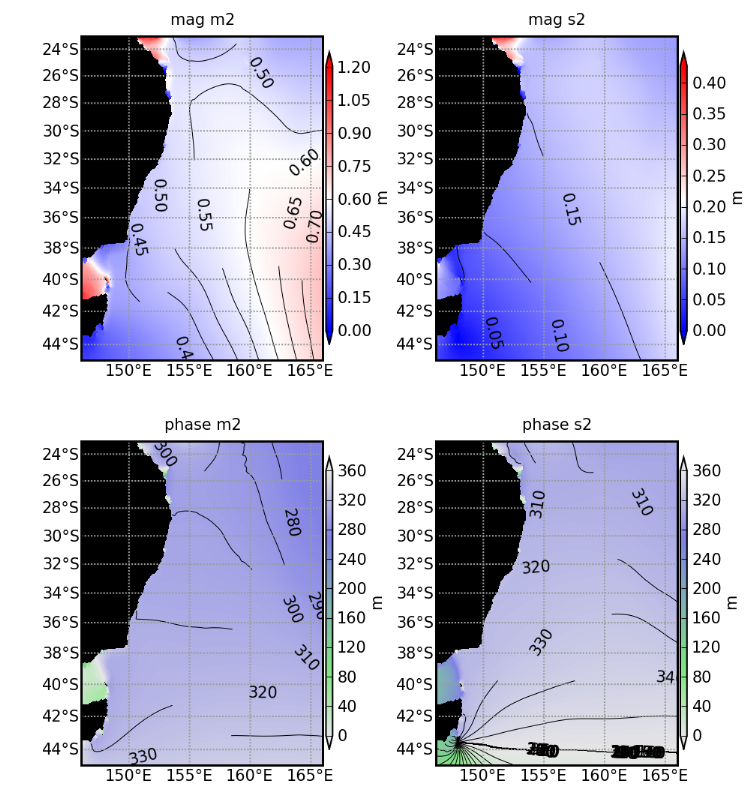
\includegraphics[width=100mm]{figures_3/otis_example.png}
\caption{Illustration of trials to implement tidal data assimilation using \OTIS{}}
\label{fig:OTIS_eg}
\end{center}
\end{figure}


The end point to this study will involve quantitative evaluation of \OGCM{} simulations carried out to assess the impact of candidate tidal solutions.










\newpage
\subsection{Sensitivity to tidal body forcing implementations in an \OGCM{}}
\label{S:plan_bodyforcing}


\subsubsection{Problem and motivation}

The prospect of explicitly resolving ocean tides within an operational \OGCM{}s raises many issues of numerical implementation. For this study, the treatment of the tidal body forcing is investigated.\\  
Practical formulations of the body forcing require some compromise - discussed in Section \ref{S:ATGP_extras}).   It is not unreasonable to expect that the simulated ocean response could show sensitivity to the details of this formulation; perhaps especially so given the significance of resonance phenomena to ocean tides \citep{Muller:2008hs}.\\



At face value the tidal body forcing implemented in \MOM{} appears overly simplistic [Section \ref{S:numerical_impl}].  However, the practical significance of body forcing nuances are not well understood.  \\
The following aspects of body force implementation within \MOM{} are raised:
\begin{inparaenum}[(a)]
\item order and degree of spatial spherical harmonics;
\item formulation of temporal variation of $c_{nm}(t)$ (harmonic versus direct);
\item treatment of SAL
\item opportunities for forcing adjustments derived from data assimilative tide models.
\end{inparaenum}

Techniques and results associated with global tidal atlases are pertinent to addressing these topics.\\



In addressing the significance of body forcing formulations, the following research questions are posed:
\begin{itemize}
\item How does a contemporary pre-computed tidal SAL field compare to the scalar approximation implemented in \MOM{}?
\item How does $\eta_{eq}$ field differ when derived directly from numerical ephemerides compared to approximation implemented in \MOM{}?
\item Is implementation of pre-calculated tidal forcing fields into \MOM{} feasible within the split-explicit configuration?
\item Can a time-domain force adjustment be derived from the GI process of the \OTIS{} software?  And if so, can it offer any value to \MOM{}?
\end{itemize}



% SAL
Within the global ocean tide modelling literature, representation of self attraction and loading (SAL) has been identified as a significant and challenging detail since the mid-1970s \cite[pp189]{Cartwright:2000tt}.
Methods have been developed to deal with the complication of the recursive dynamics of ocean mass distribution and earth elasticity.   For the sake of computational simplicity, models such as \MOM{} have employed the simple scalar parameterisation as a modification to basic body forcing.\\
The scalar parameterisation appears to be an unnecessarily blunt compromise given the current availability of pre-computed global tide solutions.  Pre-computation offers more realistic representations of SAL \citep{Egbert:2002ug}.   But for an \OGCM{} this proposition raises questions of technical implementation.  Moreover, whilst a proper treatment of SAL is understood to be very important for global tides, the relevance to \OGCM{}s or any regional ocean model is not well-established.  



% temporal 
Temporal representation of the \ATGP{} was discussed in Section \ref{S:ATGP}.   Particular technical issues arise in connection to the barotropic forcing in \MOM{}.  For instance, the manner in which split-explicit scheme is implemented in connection to surface flux fields is not amenable to direct temporal formulations of the \ATGP{}.  Despite the apparent barrier, applying arbitrary pre-computed 2-dimensional force fields within the barotropic solver may be required to address modifications under discussion.  \\
It is noted that this temporal issue is not only relevant to the \ATGP{} and SAL.  Barometric pressure forcing is formulated identically and implementation is a closely related problem to explicit tides.\\



% OTIS
A more speculative question related to body forcing is raised in connection to the `weak constraint' data assimilation process of \OTIS{}.  
The generalised inverse method in \OTIS{} effectively calculates an adjustment to the body forcing in order to account for sources of mis-representation in the tide model.  Within the use of \OTIS{} this is presented as an objective trade-off between imperfect dynamics and imperfect observations.  The proposal here is to extract the forcing adjustment from \OTIS{} and use it to adjust forcing in a separate ocean model; namely \MOM{}.  Details of grid discretisation and bathymetry are important considerations in establishing applicability.\\
Associated technical challenges will be addressed. For instance, the translation of quantities from tidal spectral space to discrete time-stepping.\\



\subsubsection{Sources}
Boundary conditions and forcing fields; \\
Observations for evaluation.   Primarily, tide gauges

This work will require technical proficiency with both the data assimilating tide mode \OTIS{} [Figure \ref{fig:OTIS_eg}] as well as the primitive equation ocean model \MOM{}.\\
Observational verification will be employed using both tide gauges and radar altimeter results.  It is proposed that the coastal altimetric research products from the French agency CTOH will be of value and registration for use of this data has been completed.
%\citep{Schiller:2007gk}
%\citep{Egbert:2002ug}
%\citep{Stepanov:2004up}


\subsubsection{Method outlook}
This study will leverage capability developed towards the study outlined in Section \ref{S:plan_OTIS}; including a regional configuration of \OTIS{} and \MOM{}.  Again, the possible alternative of employing \ROMS{} is flagged.\\



Firstly, basic preparation and comparison of several spatial fields will be carried out.   This will include relevant candidates for the  \ATGP{}, SAL and \OTIS{}-derived body forcings.   Characterisation with regard to relative magnitude and phase differences will provide an initial appreciation of possible significance.\\



Secondarily, a simplified `cheap' configuration of the \OGCM{} will be employed to investigate questions of the forcing implementation.   
In this regard two basic approaches are highlighted:
\begin{inparaenum}[(a)]
\item modification of the present harmonic formulation calculated `on the fly' within the barotropic loop;
\item application of arbitrary pre-calculated fields to the barotropic solver.
\end{inparaenum}


In light of the preceding steps, a carefully selected set of \OGCM{} simulations will be developed and evaluated against observations. 



Ultimately this study aims to contribute to understanding the significance, or otherwise, of tidal body forcing formulations and inform future operational developments. 





\newpage
\subsection{Tides and data assimilation in operational meso-scale ocean prediction}
\label{S:plan_DA}

Following the conceptual path between tidal harmonics and operational oceanography, it is pertinent to address the implications for data assimilation (DA).\\
A critical discussion of issues and prospects in this area is proposed as a concluding chapter.\\


\subsubsection{Overview of a critical discussion}
Prediction systems in the \GODAE{} heritage have intentionally excluded ocean tides to focus on mesoscale ocean turbulence [Section \ref{S:operational_oceanography}].  This approach has largely been guided and enabled by the assimilation of sea level anomaly (SLA) observations from nadir-looking altimeters.  
However, the very existence of realtime SLA datastreams has been enabled by global tide solutions founded on the historical record of observations from the same satellite platforms.\\
Thus DA has played two distinct and complimentary roles:
\begin{itemize}
\item historical observations to optimise global atlases of stationary tides \citep{Egbert:1996vr};
\item realtime observations to constrain mesoscale \OGCM{} forecasts. 
\end{itemize}


\BoxBegin
Given the prospect of explicitly resolving tidal dynamics in an \OGCM{}, how should data assimilation be approached with regard to operational sea level forecasts? \\
\BoxEnd

The motivation is summarised as follows:
\begin{enumerate}
\item it is desirable to include ocean tides in the \OGCM{} (more physical representation of barotropic conversion and mixing dynamics - Section \ref{S:tides_ogcm});
\item the skill of mesoscale ocean forecasts is reliant on DA and the contemporary global observing array;
\item naively extending the present \OGCM{} data assimilation to ingest SSH does not appear viable (tidal phase errors are likely to be more powerful than the targeted nontidal signal); 
\item the goal of simultaneously resolving ocean tides \emph{and} constraining mesoscale circulation invites a high level exploration of limitations and options.
\end{enumerate}

%require a re-evaluation of data assimilation approach.
%\item Naively introduced, explicit tidal resolution in the model would not be compatible with data assimilation due to the relative power and high frequencies of this component of sea level. 

The existing DA configuration of \BL{} (BODAS EnOI)  will provide the launching point for this discussion.  From the outset, the role of resolving tidal dynamics will be considered a tool to improve the nontidal ocean state estimation. \\




For instance, the follow sketch outlines a prospective hybrid approach, persisting with the concept of decomposing the ocean state into tidal and nontidal.\\
DA could be facilitated by employing two parallel instances of the \OGCM{}: one with full dynamics and another with only tidal forcing.   Drawing on an analogy with the UK storm tide service \cite{Horsburg:2009ui}, the difference between the models could provide a self-consistent estimate of sea level anomaly.\\
Key to this concept is the reality that representation of tidal dynamics in an \OGCM{} will always be compromised compared to best available tidal atlases. 

For instance, at each analysis step:   
\begin{inparaenum}[(i)]
\item full background state from tide-resolving \OGCM{} stepped forward in time;
\item complimentary tidal background from a tide-only version of the same \OGCM{} stepped forward in time;
\item difference states to give nontidal state estimate;
\item increments to nontidal ocean state derived from existing DA software;
\item reconstitute the full ocean state by superposition of updated nontidal state with best estimate tide prediction.
\end{inparaenum}




Supporting the discussion of prospective approaches, this discussion will draw on relevant literature and address questions such as:
\begin{itemize}
\item Are fundamental scale limits imposed by the observation array? \\
\item Would realistic changes to the observation array dictate the choice of approach? 
\item Do model parameterisations and the role bathymetry influence the balance of considerations?
\item Can the respective strengths of tidal and nontidal DA be exploited in a hybrid approach? 
\end{itemize}
































